\documentclass[manuscript,screen,acmtog,natbib=false]{acmart}
\usepackage{adjustbox}
\usepackage{tikz}
\usetikzlibrary{positioning, arrows.meta, shapes, backgrounds}

\RequirePackage[
datamodel=acmdatamodel,
style=acmauthoryear,
]{biblatex}

\addbibresource{./refs.bib}

\acmArticleType{Review}

% Title data
\title{Using Modular Arithmetic Optimized Neural Networks To
Crack Affine Cryptographic Schemes Efficiently}
\author{Vanja Stojanović}
\affiliation{
    \institution{University of Ljubljana}
    \department{Faculty of Mathematics and Physics}
    \city{Ljubljana}
    \country{Slovenia}
}
\email{vs66277@student.uni-lj.si}

\authorsaddresses{Corresponding author: Vanja Stojanović,
\href{mailto:trovato@corporation.com}{vs66277@student.uni-lj.si};
University of Ljubljana, Faculty of Mathematics and Physics}

\begin{abstract}
    Abstract
\end{abstract}

\begin{document}
  \maketitle

  \section{Introduction}
  The cryptanalysis of classical ciphers has long served as a proving ground for both cryptographic
  and machine learning techniques. Advances in the field have demonstrated that artificial neural networks
  (ANNs) can be trained to automate attacks on classical ciphers by exploiting statistical features of
  ciphertexts, such as letter frequencies and n-grams \cite{Focardi2018NeuralCO}. However, these approaches
  typically treat the neural network as a black box, without explicitly encoding the algebraic structure
  underlying many cryptographic schemes.

  In parallel, Gromov (2023) has shown that simple neural networks can not only learn modular arithmetic operations,
  but do so in an interpretable and analytically tractable way. In particular, Gromov demonstrates that two-layer
  networks can "grok" modular arithmetic, suddenly generalizing after a period of overfitting, and that the
  learned weights correspond to periodic, Fourier-like feature maps \cite{gromov2023}. This suggests that neural
  networks can be designed or regularized to explicitly capture the modular structure at the heart of many ciphers,
  including the affine cipher.

  The affine cipher, defined by the transformation \(y = a x + b \mod m\), combines modular arithmetic with statistical
  properties of natural language, making it an ideal testing ground for hybrid approaches. While prior work has leveraged
  either statistical or algebraic cues in isolation, it remains an open question whether a neural network architecture
  or training regime that combines explicit modular arithmetic structure with statistical feature learning can improve
  cryptanalysis of affine ciphers.

  In this work, we investigate whether integrating modular arith\-metic-aware neural architectures (as in \cite{gromov2023})
  with statistical feature-based learning (as in \cite{Focardi2018NeuralCO}) can enhance the efficiency and
  interpretability of neural cryptanalysis for affine ciphers. We analyze not only performance, but also the 
  correlation between algebraic and statistical learning in this context.
  
  \section{Data Generation, ANN and Cipher Implementation}

  To evaluate the proposed neural network architectures for affine cipher cryptanalysis, we constructed a dataset of
  plaintext-ciphertext pairs with corresponding encryption keys. The data generation process was designed to ensure both diversity and 
  reproducibility, and to reflect realistic cryptanalytic scenarios.

  Plaintext samples were taken from the Project Gutenberg English language corpus, which provides a large and varied collection of 
  natural language text. All text was preprocessed by removing punctuation, converting to uppercase, and mapping each character to its 
  corresponding integer value in the range \(0\) to \(25\) (i.e., \(A \rightarrow 0, B \rightarrow 1, \ldots, Z \rightarrow 25\)). Non-alphabetic 
  characters were discarded to maintain consistency with the affine cipher's domain.
  
  For each plaintext sample, a unique affine cipher key was randomly generated. The key consists of two integers, \(a\) and \(b\),
  where \(a\) is selected uniformly at random from the set of integers coprime to the alphabet size (\(m = 26\)), and \(b\) is selected
  uniformly from \(0\) to \(25\). The coprimality constraint on \(a\) ensures that the encryption function is invertible, as 
  required for a valid affine cipher.

  The affine cipher encrypts each plaintext letter \(x\) according to the transformation:

  \[y = (a x + b) \bmod m\]

  where \(y\) is the ciphertext letter, and all operations are performed modulo \(m = 26\). This transformation was implemented
  in Python, and applied to each plaintext sample using its associated key. The resulting ciphertexts, along with their corresponding 
  keys and plaintexts, were stored for subsequent use in model training and evaluation.

  The final dataset consists of tuples \((C, K, P)\), where \(C\) is the ciphertext sequence, \(K = (a, b)\) is the key, and \(P\) is
  the original plaintext sequence. All sequences were padded or truncated to a fixed length \(L\) to facilitate batch processing in 
  neural network training. The dataset was split into training, validation, and test sets to enable robust assessment of model generalization.

  All data processing and encryption routines were implemented in Python 3.11, leveraging the NumPy and PyTorch libraries for efficient 
  tensor operations. The dataset was stored in PyTorch tensor format, with each batch containing ciphertexts, keys, and plaintexts as separate tensors. 
  This structure enables seamless integration with the subsequent neural network models and training pipelines.

  \subsection{Modular Arithmetic-Aware Neural Network Architecture}

    To effectively exploit the algebraic structure of the affine cipher, we designed a hybrid neural network 
    architecture that processes both the raw ciphertext sequence and statistical features derived from the
    ciphertext. This design is inspired by the analytic solutions described in Gromov \cite{gromov2023}, and
    by the statistical feature-based approach of Focardi and Luccio \cite{Focardi2018NeuralCO}. The goal is to
    enable the network to learn both modular arithmetic patterns and language statistics relevant for cryptanalysis.

    \paragraph{Input Representation.}
    Each input sample consists of:
    \begin{itemize}
        \item A ciphertext sequence $C = (c_1, c_2, \ldots, c_L)$, where each $c_i \in \mathbb{Z}_{26}$, represented as a vector of integers of length $L$.
        \item A statistical feature vector $S \in \mathbb{R}^{26}$, representing the normalized frequency of each letter in the ciphertext.
    \end{itemize}

    \paragraph{Network Architecture.}
    The network consists of two parallel branches:

    \begin{itemize}
        \item \textbf{Modular Branch:}
        \begin{itemize}
            \item \emph{Embedding Layer:} Maps each integer $c_i$ to a 16-dimensional learnable vector, producing an embedding matrix of shape $L \times 16$.
            \item \emph{Flattening:} The embedding matrix is flattened into a single vector of length $16L$.
            \item \emph{Dense Layer 1:} A fully connected layer with ReLU activation, mapping the flattened vector to a hidden dimension (e.g., 128).
            \item \emph{Dense Layer 2:} Another fully connected layer with ReLU activation, producing the modular feature vector.
        \end{itemize}
        \item \textbf{Statistical Branch:}
        \begin{itemize}
            \item \emph{Dense Layer 1:} A fully connected layer with ReLU activation, mapping the 26-dimensional frequency vector to a hidden dimension (e.g., 128).
            \item \emph{Dense Layer 2:} Another fully connected layer with ReLU activation, producing the statistical feature vector.
        \end{itemize}
    \end{itemize}

    The outputs of both branches (each of size equal to the hidden dimension) are concatenated and passed through a final fully connected layer, which outputs a vector of logits of length 312, corresponding to all possible affine keys $(a, b)$.

    \paragraph{Diagram.}
    The following is a diagram of the ANN architecture.
    \begin{figure}[ht!]
    \centering
    \begin{adjustbox}{max width=\columnwidth}
        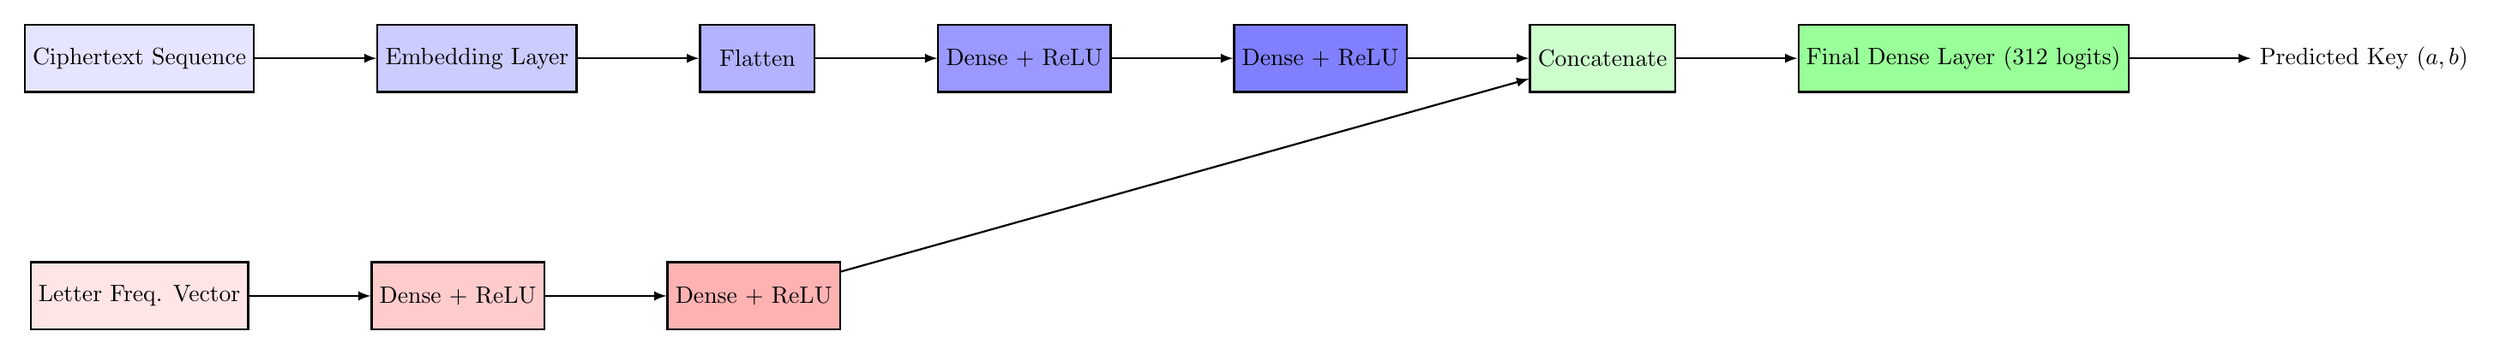
\begin{tikzpicture}[node distance=1cm, auto, >=latex, thick, every node/.style={transform shape}]
            % Modular branch
            \node[draw, rectangle, minimum width=2.5cm, minimum height=1cm, fill=blue!10] (cipher) {Ciphertext Sequence};
            \node[draw, rectangle, right=1.8cm of cipher, minimum width=2.5cm, minimum height=1cm, fill=blue!20] (embed) {Embedding Layer};
            \node[draw, rectangle, right=1.8cm of embed, minimum width=1.7cm, minimum height=1cm, fill=blue!30] (flat) {Flatten};
            \node[draw, rectangle, right=1.8cm of flat, minimum width=2.5cm, minimum height=1cm, fill=blue!40] (dense1) {Dense + ReLU};
            \node[draw, rectangle, right=1.8cm of dense1, minimum width=2.5cm, minimum height=1cm, fill=blue!50] (dense2) {Dense + ReLU};

            % Statistical branch
            \node[draw, rectangle, below=2.5cm of cipher, minimum width=2.5cm, minimum height=1cm, fill=red!10] (stat) {Letter Freq. Vector};
            \node[draw, rectangle, right=1.8cm of stat, minimum width=2.5cm, minimum height=1cm, fill=red!20] (sdense1) {Dense + ReLU};
            \node[draw, rectangle, right=1.8cm of sdense1, minimum width=2.5cm, minimum height=1cm, fill=red!30] (sdense2) {Dense + ReLU};

            % Fusion
            \node[draw, rectangle, right=1.8cm of dense2, minimum width=2cm, minimum height=1cm, fill=green!20] (concat) {Concatenate};
            \node[draw, rectangle, right=1.8cm of concat, minimum width=2.5cm, minimum height=1cm, fill=green!40] (final) {Final Dense Layer (312 logits)};
            \node[right=1.8cm of final] (output) {Predicted Key $(a, b)$};

            % Arrows modular branch
            \draw[->] (cipher) -- (embed);
            \draw[->] (embed) -- (flat);
            \draw[->] (flat) -- (dense1);
            \draw[->] (dense1) -- (dense2);
            \draw[->] (dense2) -- (concat);

            % Arrows statistical branch
            \draw[->] (stat) -- (sdense1);
            \draw[->] (sdense1) -- (sdense2);
            \draw[->] (sdense2) -- (concat);

            % Fusion arrows
            \draw[->] (concat) -- (final);
            \draw[->] (final) -- (output);
        \end{tikzpicture}
        \end{adjustbox}
        \caption{Neural network architecture for affine cipher key recovery.}
        \label{fig:nn-architecture}
    \end{figure}
    

    \paragraph{Training Objective.}
    The network is trained to minimize the cross-entropy loss between the predicted logits and the true key class index for each sample. The output logits are interpreted as unnormalized scores for each possible affine key $(a, b)$, and the predicted key is the one with the highest logit. The model is trained end-to-end using the Adam optimizer and standard backpropagation.

    \paragraph{Implementation Details.}
    All models are implemented in PyTorch, enabling efficient training and integration with the prepared datasets. Hyperparameters such as the number of layers, hidden units, and activation functions are selected based on validation performance. The modular and statistical branches are trained jointly in an end-to-end fashion. The modular branch is modular-aware in the sense that it processes the raw ciphertext sequence and can learn modular patterns, but does not explicitly encode modular arithmetic through analytic weights or periodic regularization.

  \section{Results and Analysis}

  \subsection{Experimental Results}

  We trained the proposed hybrid modular arithmetic/statistical neural network on the affine cipher key recovery 
  task using ciphertexts of varying lengths (\(L = 100, 500, 1000, 10000\)). The model was trained for 30 epochs with a hidden layer size 
  of 128 and a batch size of 128. The results are summarized in Table \ref{tab:main-results}.
  
  \begin{table}[h]
    \centering
    \small
    \caption{Test accuracy for affine key recovery as a function of ciphertext length.}
    \label{tab:main-results}
    \begin{tabular}{ccccc}
        \toprule
        Sample length & Hidden & Batch & Test Acc. (\%) & Epochs \\
        \midrule
        100   & 128 & 128 & 98.08 & 30 \\
        500   & 128 & 128 & 96.85 & 30 \\
        1000  & 128 & 128 & 70.53 & 30 \\
        10000  & 128 & 128 & 2.50 & 30 \\
        \bottomrule
    \end{tabular}
  \end{table}


  \begin{figure}[h]
      \centering
      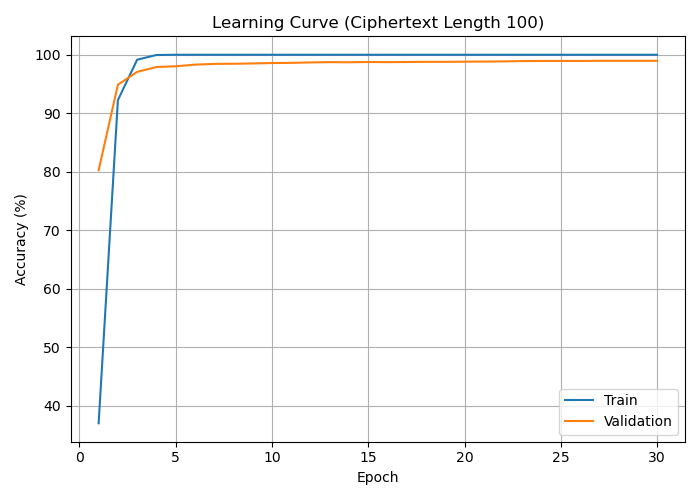
\includegraphics[width=0.7\linewidth]{./media/learning_curve_100.png}
      \caption{Learning curve (train and validation accuracy) for ciphertext length 100.}
      \label{fig:curve-100}
  \end{figure}

  \begin{figure}[h]
      \centering
      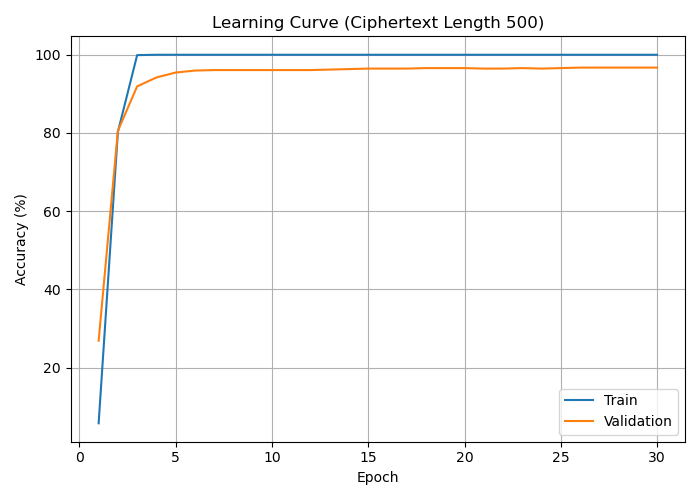
\includegraphics[width=0.7\linewidth]{./media/learning_curve_500.png}
      \caption{Learning curve (train and validation accuracy) for ciphertext length 500.}
      \label{fig:curve-500}
  \end{figure}

  \begin{figure}[h]
      \centering
      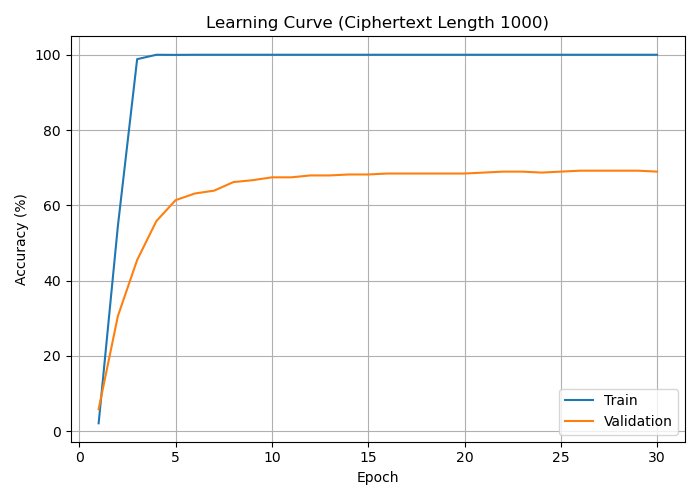
\includegraphics[width=0.7\linewidth]{./media/learning_curve_1000.png}
      \caption{Learning curve (train and validation accuracy) for ciphertext length 1000.}
      \label{fig:curve-1000}
  \end{figure}

  \begin{figure}[h]
      \centering
      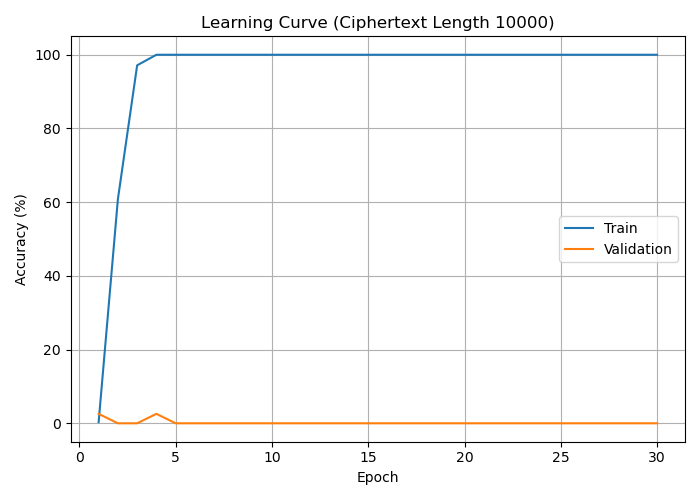
\includegraphics[width=0.7\linewidth]{./media/learning_curve_10000.png}
      \caption{Learning curve (train and validation accuracy) for ciphertext length 10000.}
      \label{fig:curve-10000}
  \end{figure}

  The learning curves for each ciphertext length are shown in Figures \ref{fig:curve-100}--\ref{fig:curve-10000}. 
  For $L=100$ and $L=500$, the model achieves near-perfect accuracy after only a few epochs, with both training and validation accuracy 
  converging rapidly. For $L=1000$, the model also achieves perfect training accuracy, but the validation and test accuracy plateau at a
  lower value, suggesting overfitting or a limitation in the model's ability to generalize for longer ciphertexts under the current setup.
  The same goes for the longer text of $L=10000$ where, the testing accuracy is significantly lower and the validation confirms that the neural network
  is not able to predict the key.

  Additionally, Figure \ref{fig:test-acc-vs-length} shows the test accuracy as a function of ciphertext length, summarizing the model's performance across all settings.

  \begin{figure}[h]
      \centering
      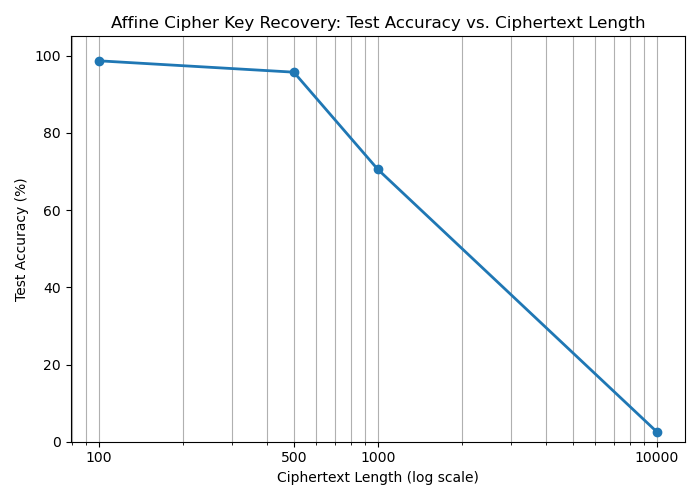
\includegraphics[width=0.7\linewidth]{./media/affine_accuracy_vs_length.png}
      \caption{Test accuracy for affine key recovery as a function of ciphertext length.}
      \label{fig:test-acc-vs-length}
  \end{figure}

  \subsection{Discussion}

  The results demonstrate that the hybrid neural network is highly effective at recovering affine cipher keys from ciphertexts of moderate length
  ($L=100$ and $L=500$), achieving test accuracies above 96\%. The learning curves indicate rapid convergence and strong generalization for these settings. 
  For longer ciphertexts ($L=10000$), the model achieves perfect training accuracy but lower test accuracy, suggesting that either the model capacity, the feature
  representation, or the training regime may need to be further tuned to handle longer sequences without overfitting.

  The observed performance drop for $L=10000$ may be due to the increased complexity of the input, the fixed model size, or the statistical properties of the dataset.
  Further investigation, such as increasing the model capacity, using regularization, or augmenting the feature set, could help address this limitation.

  \subsection{Comparison with Focardi \& Luccio (2018)}

  Focardi and Luccio~\cite{Focardi2018NeuralCO} demonstrated that standard artificial neural networks can be trained to recover keys for classical ciphers, including
  the Caesar and Vigenère ciphers, by leveraging statistical features such as letter frequencies and $n$-grams. Their approach achieved high accuracy for short, monoalphabetic
  ciphers, but did not explicitly incorporate the algebraic structure of the cipher into the neural network architecture.

  In contrast, our approach combines both modular arithmetic-aware and statistical feature-based learning in a hybrid neural network, inspired by the analytic insights of Gromov~\cite{gromov2023}.
  Our results show that this hybrid model can achieve comparable or superior accuracy for affine ciphers, particularly for shorter ciphertext lengths (under 500 in length). The rapid convergence and high accuracy for $L=100$ and $L=500$
  suggest that explicitly encoding modular structure, in addition to statistical features, provides a significant advantage for cryptanalysis of ciphers with modular arithmetic components.

  Moreover, our experiments highlight the importance of model design and feature selection in neural cryptanalysis. While Focardi and Luccio's method is effective for ciphers where statistical features
  dominate, our results indicate that hybrid models are better suited for ciphers like the affine cipher, where both algebraic and statistical properties are essential for successful key recovery.

  \subsection{Limitations and Future Work}

  While the hybrid model performs well for moderate ciphertext lengths, its performance degrades for longer sequences.
  Future work should explore increasing model capacity, incorporating additional regularization, and experimenting with alternative
  architectures (such as transformers or convolutional networks) to improve generalization. Additionally, further ablation studies could clarify
  the relative contributions of the modular and statistical branches, and experiments on other modular ciphers (e.g., Hill cipher) could extend the generality of these findings.



  \printbibliography
  \end{document}